\section{Risikoanalyse}

Risiken werden während der Projektplanung ebenfalls eruiert und tabellarischkategorisiert. Dabei werden ebenfalls Folgerisiken und Dringlichkeit beurteilt. Um diesen Risiken entgegenzuwirken werden Präventionsmassnahmen ausgearbeitet und implementiert. 
\\
\\
\\
\\
\\

\begin{figure}[H]
	\centering
	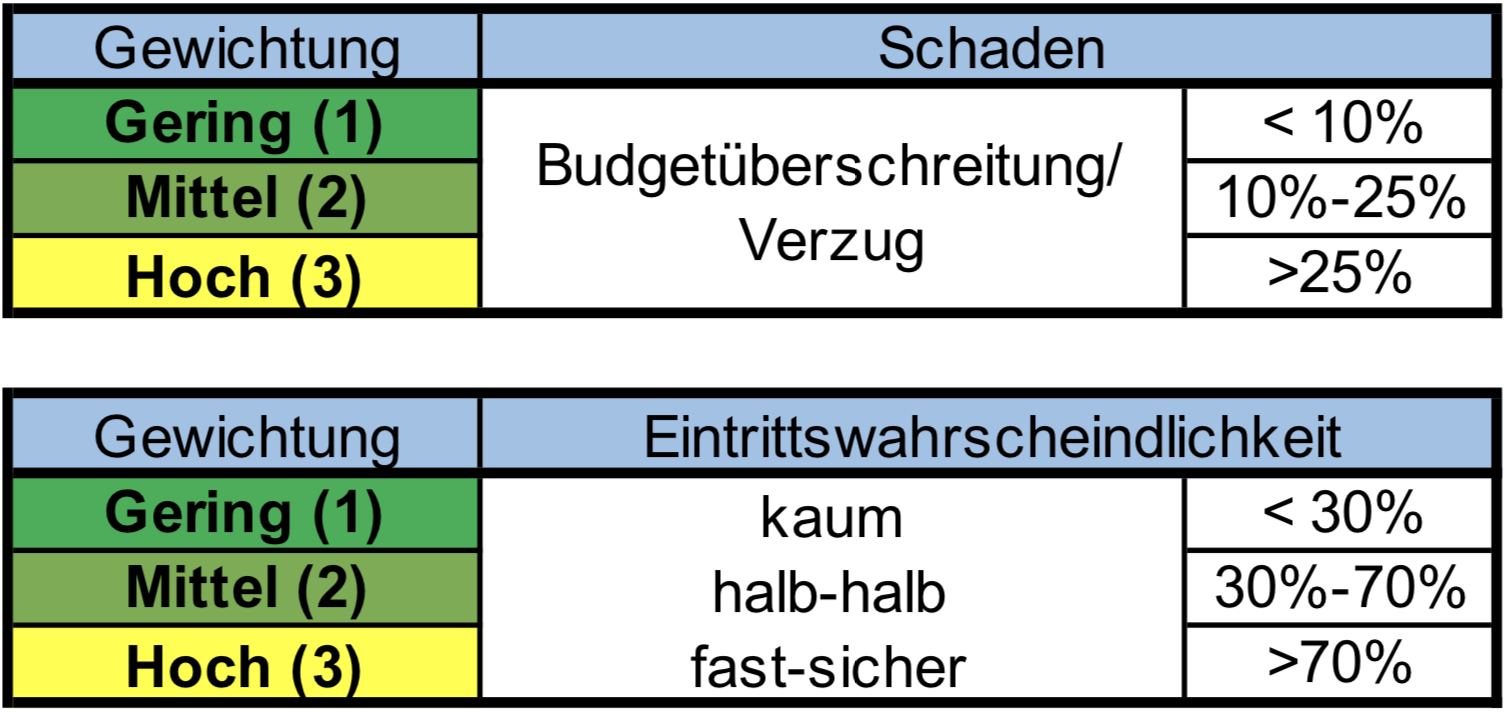
\includegraphics[width=14cm]{Gewichtung_P2.png}
	\label{fig:Gewichtung}
\end{figure}

\newpage



\begin{figure}[H]
\centering
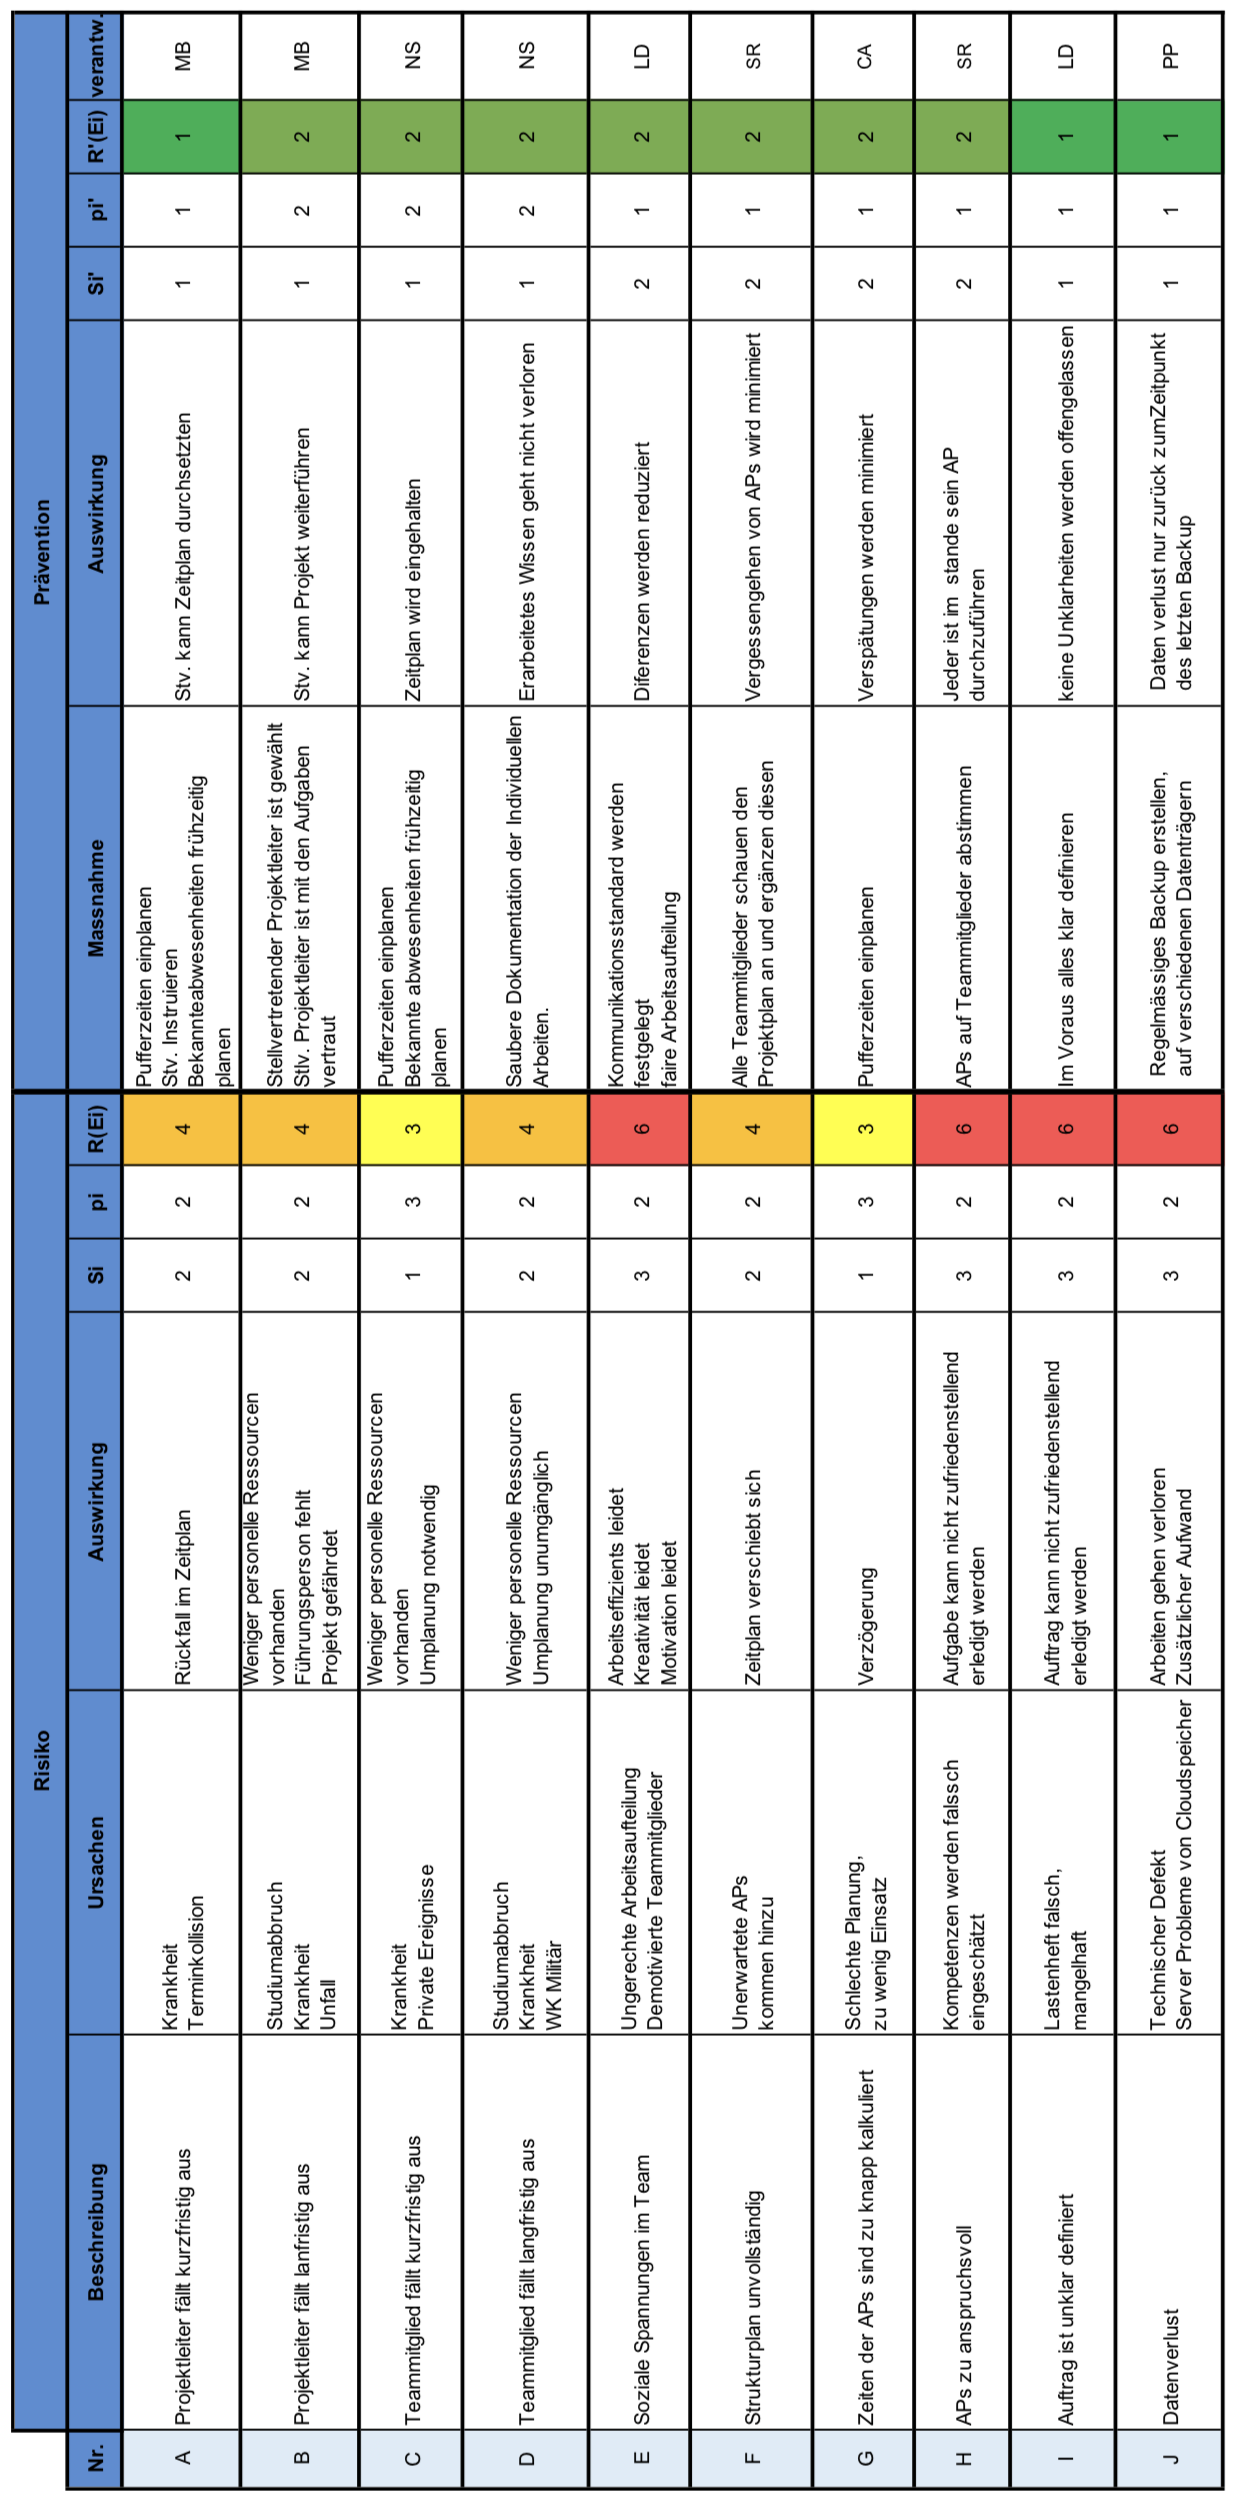
\includegraphics[width=12.5cm]{Risikotabelle_P2.png}
\label{fig:Risikotabell}
\end{figure}

\newpage
\begin{figure}[H]
	\centering
	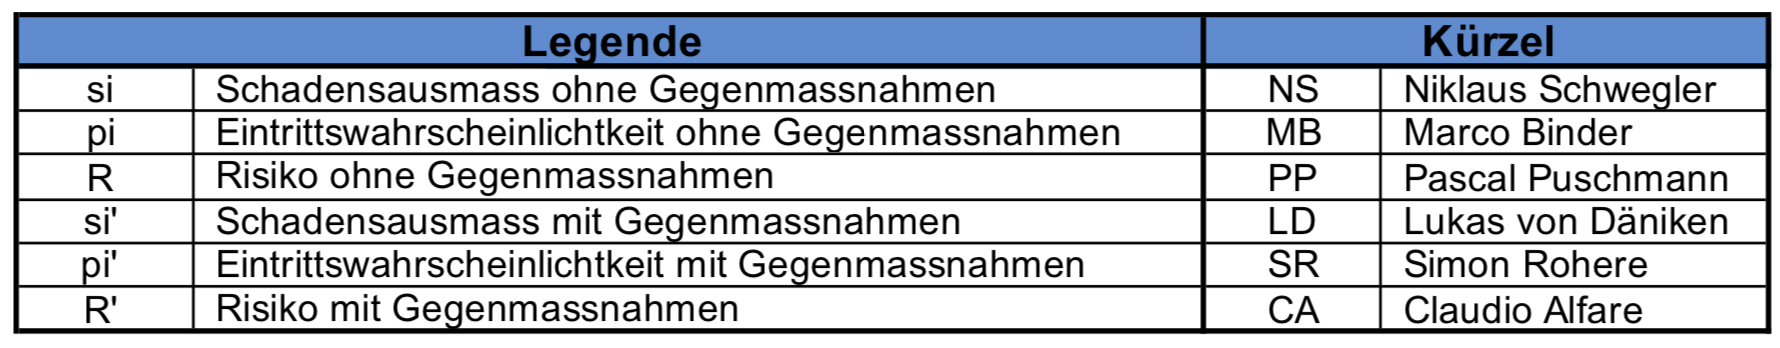
\includegraphics[width=14cm]{Legende_P2.png}
	\label{fig:Tabelle}
\end{figure}







Auf der folgenden Risikomap sind alle Gefahren jeweils mit und ohne Präventionsmassnahme graphisch dargestellt.

\begin{figure}[H]
	\centering
	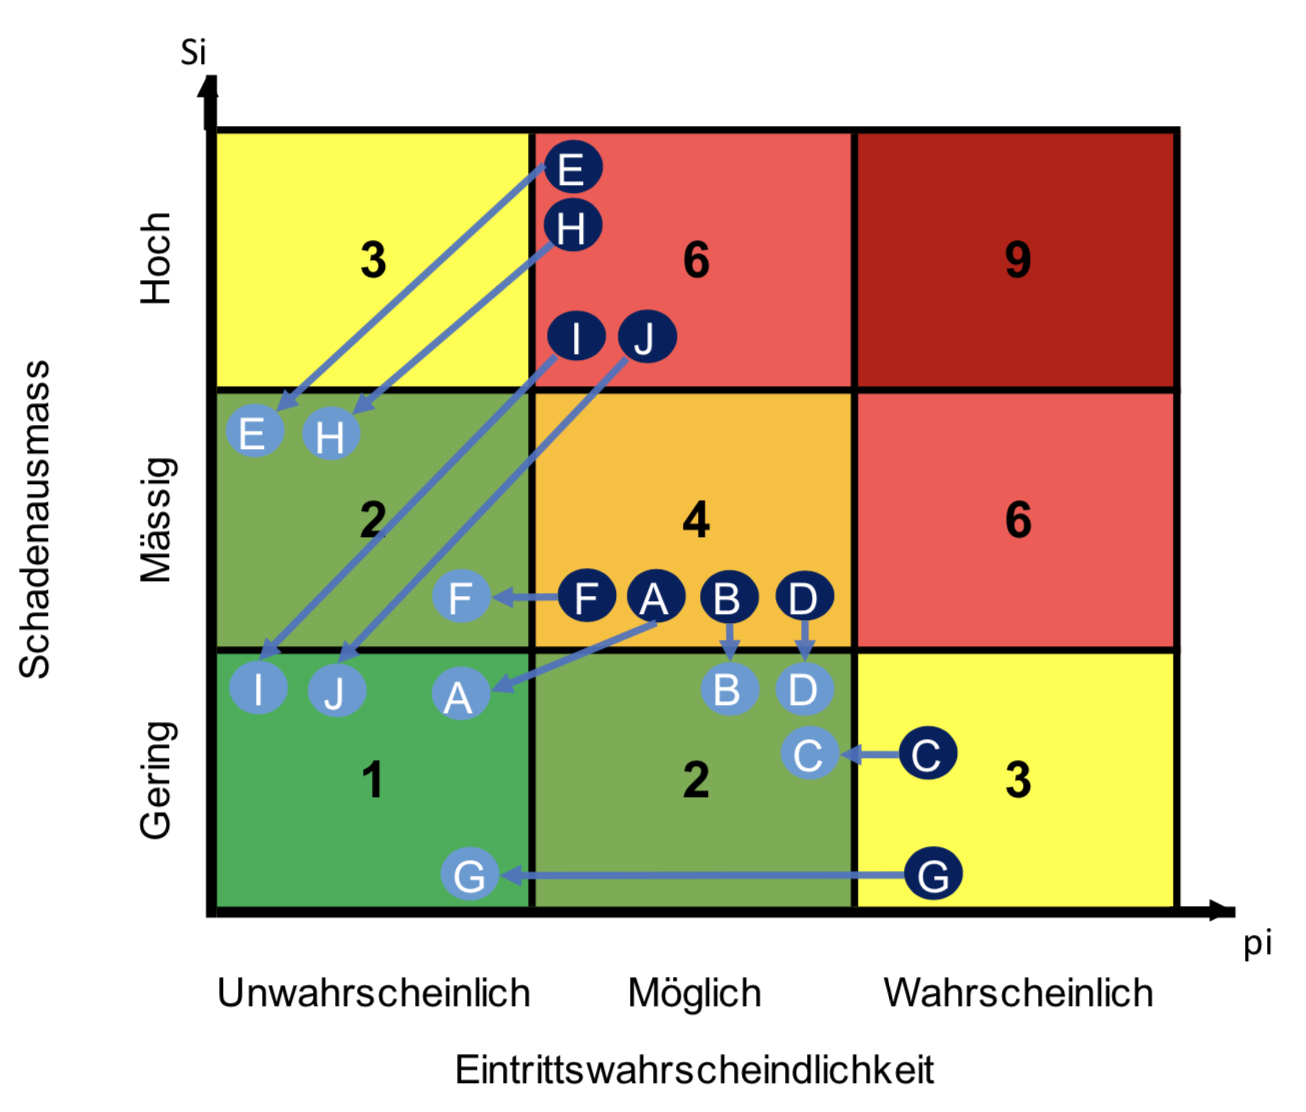
\includegraphics[width=14cm]{Matrix_verschiebung_P2.png}
	\label{fig:Matrix_verschiebung}
\end{figure}


\begin{figure}[H]
	\centering
	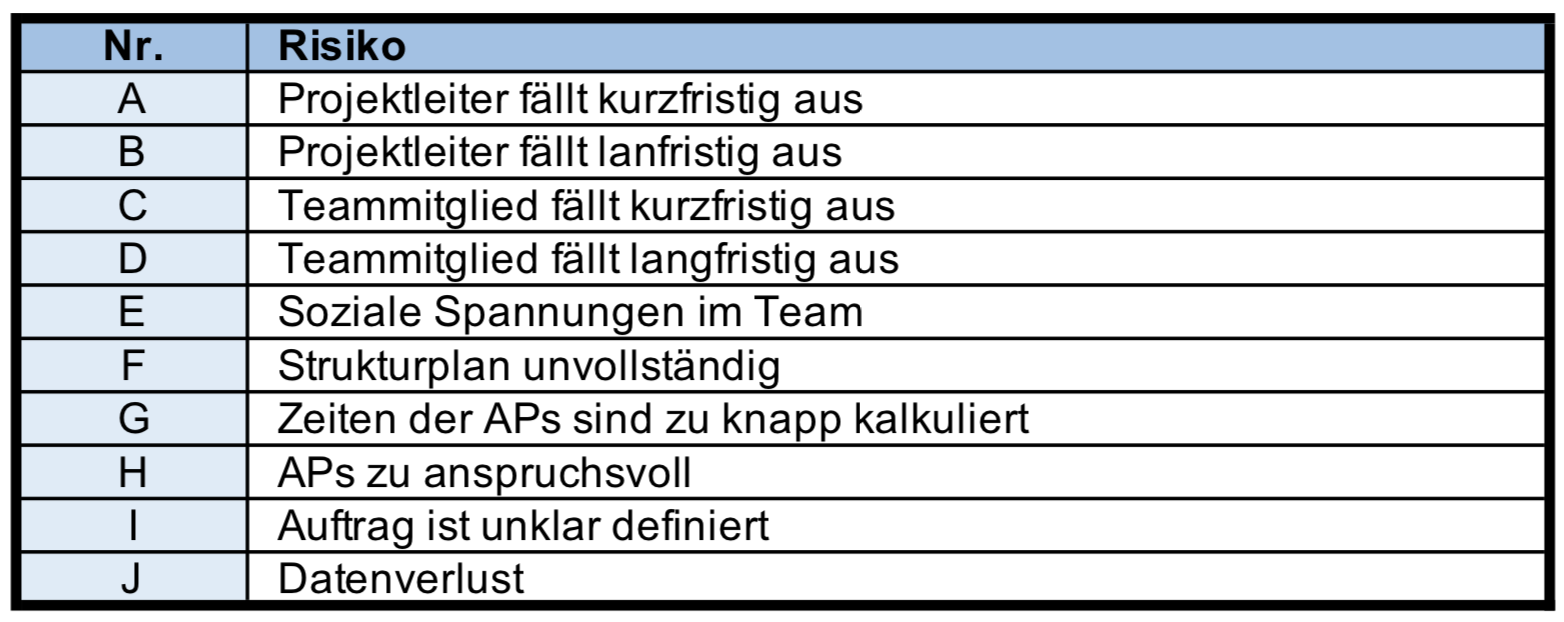
\includegraphics[width=14cm]{Risikouebersicht_P2.png}
	\label{fig:Risikoüebersicht}
\end{figure}
